\documentclass[a4paper]{report}
	\usepackage{graphicx}
	\begin{document}
		\title{End-to-End Learning for Self-Driving Cars}
		\author{Sankalp Shekhar,Lex Fridman,Sebastian Thrun}
		\date{\today}
		\maketitle
		\tableofcontents
		\newpage
		\chapter{The Journey so far}
		\section{Abstract}
		 \ref{subsec1} We trained a convolutional neural network (CNN) to map raw pixels from a sin-gle front-facing camera directly to steering commands. This end-to-end approachproved surprisingly powerful. With minimum training data from humans the sys-tem learns to drive in traffic on local roads with or without lane markings and onhighways. It also operates in areas with unclear visual guidance such as in parkinglots and on unpaved roads.The system automatically learns internal representations of the necessary process-ing steps such as detecting useful road features with only the human steering angleas the training signal. We never explicitly trained it to detect, for example, the out-line of roads.Compared to explicit decomposition of the problem, such as lane marking detec-tion, path planning, and control, our end-to-end system optimizes all processingsteps  simultaneously.   We  argue  that  this  will  eventually  lead  to  better  perfor-mance and smaller systems.  Better performance will result because the internalcomponents self-optimize to maximize overall system performance, instead of op-timizing human-selected intermediate criteria, e. g., lane detection.  Such criteriaunderstandably are selected for ease of human interpretation which doesn’t auto-matically guarantee maximum system performance.  Smaller networks are possi-ble because the system learns to solve the problem with the minimal number ofprocessing steps.We  used  an  NVIDIA  DevBox  and  Torch  7  for  training  and  an  NVIDIADRIVETMPX  self-driving  car  computer  also  running  Torch  7  for  determiningwhere to drive. The system operates at 30 frames per second (FPS).
		\newpage
		\section{Introduction}
		have revolutionized pattern recognition [2].  Prior to the widespread adoption of CNNs,most pattern recognition tasks were performed using an initial stage of hand-crafted feature extrac-tion followed by a classifier.  The breakthrough of CNNs is that features are learned automaticallyfrom training examples.  The CNN approach is especially powerful in image recognition tasks be-cause the convolution operation captures the 2D nature of images.  Also, by using the convolutionkernels to scan an entire image, relatively few parameters need to be learned compared to the totalnumber of operations.While CNNs with learned features have been in commercial use for over twenty years section,  theiradoption has exploded in the last few years because of two recent developments. First, large, labeleddata sets such as the Large Scale Visual Recognition Challenge (ILSVRC) [4] have become avail-able for training and validation.  Second, CNN learning algorithms have been implemented on themassively parallel graphics processing units (GPUs) which tremendously accelerate learning andinference.In this paper,  we describe a CNN that goes beyond pattern recognition.   It learns the entire pro-cessing pipeline needed to steer an automobile.  The groundwork for this project was done over 10years ago in a Defense Advanced Research Projects Agency (DARPA) seedling project known asDARPA Autonomous Vehicle (DAVE) [5] in which a sub-scale radio control (RC) car drove througha junk-filled alley way. DAVE was trained on hours of human driving in similar, but not identical en-vironments. The training data included video from two cameras coupled with left and right steeringcommands from a human operator.In many ways, DAVE-2 was inspired by the pioneering work of Pomerleau [6] who in 1989 built theAutonomous Land Vehicle in a Neural Network (ALVINN) system. It demonstrated that an end-to-end trained neural network can indeed steer a car on public roads. Our work differs in that 25 years ofadvances let us apply far more data and computational power to the task. In addition, our experiencewith CNNs lets us make use of this powerful technology. (ALVINN used a fully-connected networkwhich is tiny by today’s standard.)While  DAVE  demonstrated  the  potential  of  end-to-end  learning,  and  indeed  was  used  to  justifystarting the DARPA Learning Applied to Ground Robots (LAGR) program [7], DAVE’s performancewas not sufficiently reliable to provide a full alternative to more modular approaches to off-roaddriving. DAVE’s mean distance between crashes was about 20 meters in complex environments.Nine months ago, a new effort was started at NVIDIA that sought to build on DAVE and create arobust system for driving on public roads. The primary motivation for this work is to avoid the needto recognize specific human-designated features, such as lane markings, guard rails, or other cars,and to avoid having to create a collection of “if, then, else” rules, based on observation of thesefeatures. This paper describes preliminary results of this new effort.
		\subsection{Data Selection}
		\label{subsec1}	
		The  first  step  to  training  a  neural  network  is  selecting  the  frames  to  use.   Our  collected  data  islabeled with road type,  weather condition,  and the driver’s activity (staying in a lane,  switchinglanes, turning, and so forth).  To train a CNN to do lane following we only select data where thedriver was staying in a lane and discard the rest.  We then sample that video at 10 FPS. A highersampling rate would result in including images that are highly similar and thus not provide muchuseful information.
		Types of Neural Networks:
		\begin{itemize}
			\item Feed Forward Neural Network
				\begin{enumerate}
					\item Single Layered Perceptron
					\item Multi Layered Perceptron
				\end{enumerate}
			\item Convolutional Neural Network
			\item Recurrent Neural Network
			\item Generative Adversarial Network
		\end{itemize}
		\begin{figure}[h] 
			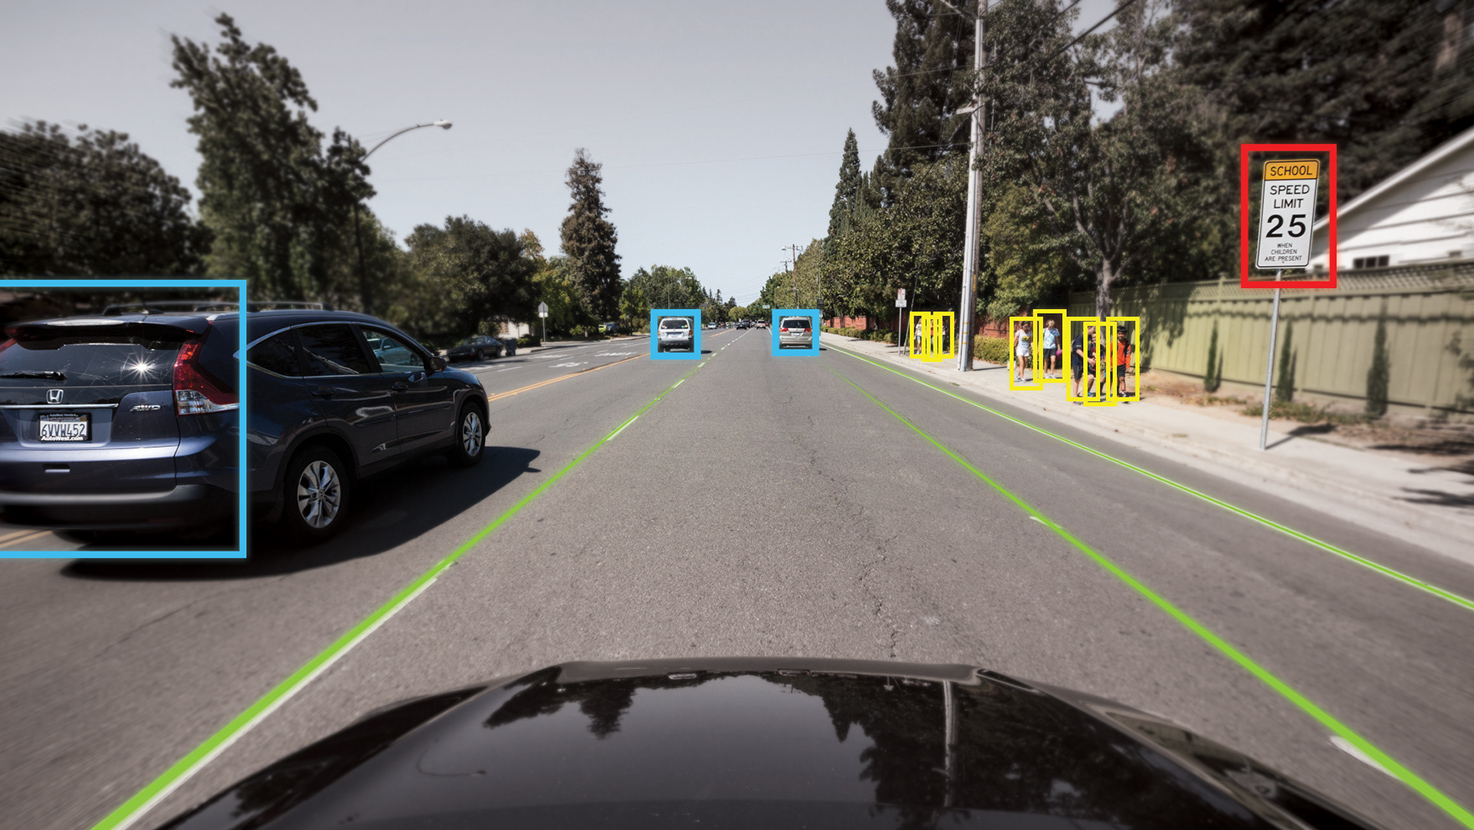
\includegraphics[width=\linewidth]{latex1.jpg}
			\caption{Lane Detection and Vehicle Recognition}
			\label{figref1}
		\end{figure}
		
		Figure \ref{figref1} shows a self driving car detecting lanes, vehicles, pedestrians, and road signs around it.
		
		
		
	
	\end{document}
	